\documentclass[12pt]{article}
\usepackage{Geoff,graphicx}

\title{Meeting notes 6-21-2017}
\author{Geoff Iyer}
\date{}

\begin{document}

\maketitle

\section{Change Detection}

Here's a brief overview of the algorithm. Given images $X,Y$ of the same size, we run the graph matching algorithm to get a permutation map $\rho: X\to Y$. We then look at the quantities
\begin{align}
  \norm{X_i - X_{\rho^{-1}(i)}} \\
  \norm{Y_i - Y_{\rho(i)}}
\end{align}
to determine the amount of change between $X$ and $Y$ on a pixel-by-pixel basis.

A new idea: instead of viewing every pixel, we restrict our attention to pixels $i$ for which the match $i \to \rho(i)$ has a large similarity in the graph match algorithm. The heuristic is that if the graph-match is considered good, but the coregistration match is considered bad, then this signifies a change between $X$ and $Y$.

\subsection{Synthetic Example}

This picture (figure \ref{fig:synthetic}) already appeared in the ATC talk. Nothing new here.

\begin{figure}
  \begin{minipage}[b]{0.40\linewidth}
    \centering
    
\includegraphics[width=\textwidth]{./dataAfter.png}
    \caption{Image $X$}
  \end{minipage}
  \hfill
  \begin{minipage}[b]{0.40\linewidth}
    \centering
    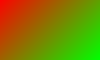
\includegraphics[width=\textwidth]{./dataBefore.png}
    \caption{Image $Y$}
  \end{minipage}
  \vfill
  \begin{minipage}[b]{0.40\linewidth}
    \centering
    
\includegraphics[width=\textwidth]{./naivediff.png}
    \caption{Naive difference $\norm{X-Y}$}
  \end{minipage}
  \hfill
  \begin{minipage}[b]{0.40\linewidth}
    \centering
    
\includegraphics[width=\textwidth]{./normMap.png}
    \caption{$\norm{x_i - x_{\rho(i)}}$}
  \end{minipage}
  \caption{Synthetic graph match example}
  \label{fig:synthetic}
\end{figure}

\subsection{Shift Example}

In this example (figure \ref{fig:shift}) we use two pictures that are nearly equivalent. Both pictures are taken from the ``before'' section of the flood data. They capture almost the same area, but are a little offset (the overlap is about 80\% of the full image). We run the graph matching algorithm, and compare the permuted pictures to the originals to get an idea of the changes.

The results are promising. Both figures have roughly the same features (two yellow patches, one black curve, and a purple background), and we managed to detect that these 3 features each moved between picture $X$ and picture $Y$.
\begin{figure}
  \makebox[\textwidth][c]{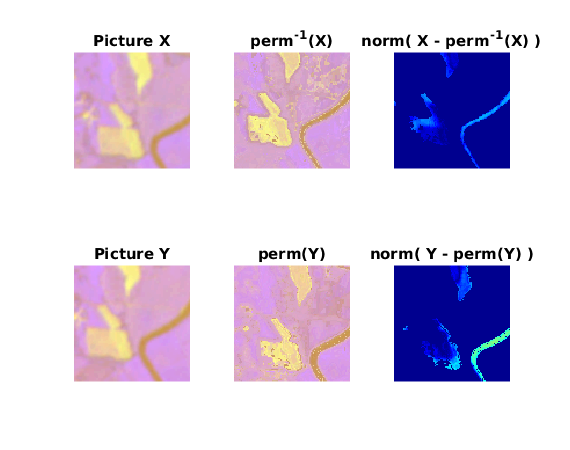
\includegraphics[width = 22cm]{changedetect_shift.png}}%
  \caption{Example Change Detection: Shift}
  \label{fig:shift}
\end{figure}

\subsection{Scaling Example}

In this example (figure \ref{fig:scaling}) the two pictures capture the same area at the same time (both are ``before'' the flood). We scale the picture $Y$, decreasing the luminosity. Theoretically, the graph match should just be the identity, and our example more or less captures this.

\begin{figure}
  \makebox[\textwidth][c]{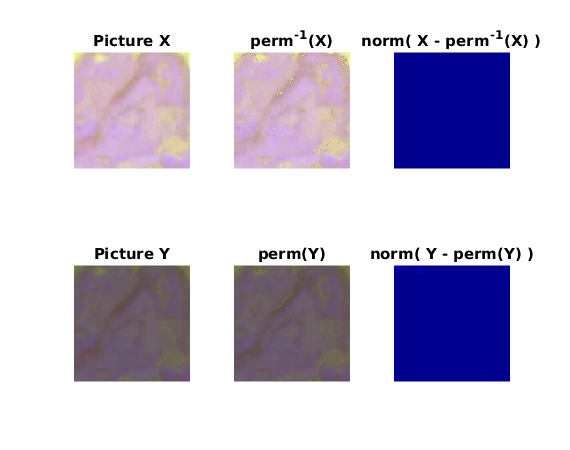
\includegraphics[width = 22cm]{changedetect_scaling.png}}%
  \caption{Example Change Detection: Scaling}
  \label{fig:scaling}
\end{figure}

\subsection{Before and After Example}

Here we show two examples where we use the ``before'' and ``after'' sections of the flood data as originally intended. In both examples, picture $X$ and $Y$ capture the exact same area. $X$ is taken before the flood, and $Y$ is taken after.

These examples are much harder for the algorithm to manage. In figure \ref{fig:beforeafterokay} we show an example where the before and after pictures are quite similar. The change detection algorithm manages to pick out some important changes, but also highlights a lot of areas where there is no significant change.

The example in figure \ref{fig:beforeafterfail} is much worse. Here there is very little change between the two pictures, other than a general change in hue. Unfortunately, the algorithm does not find this at all. The permutation $\rho: X\to Y$ is pretty ridiculous, so the algorithm finds a lot of ``changes'' where there should not be any.

\begin{figure}
  \makebox[\textwidth][c]{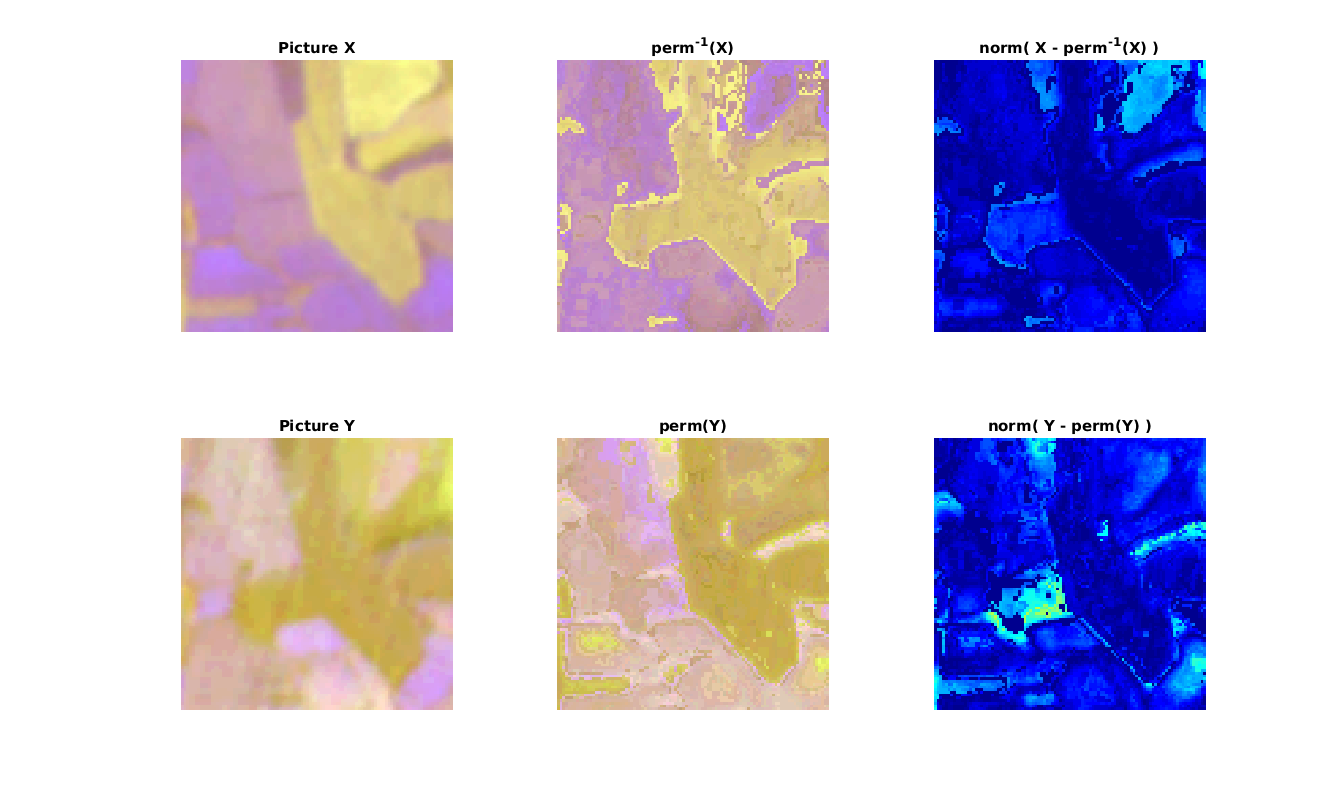
\includegraphics[width = 22cm]{changedetect_beforeafterokay.png}}%
  \caption{Example Change Detection: Before and After (okay)}
  \label{fig:beforeafterokay}
\end{figure}

\begin{figure}
  \makebox[\textwidth][c]{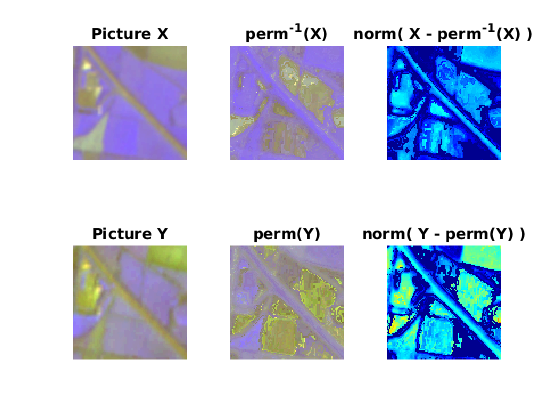
\includegraphics[width = 22cm]{changedetect_beforeafterfail.png}}%
  \caption{Example Change Detection: Before and After (fail)}
  \label{fig:beforeafterfail}
\end{figure}


\end{document}
